\documentclass[a4paper]{article}
\usepackage[a4paper, margin=2cm]{geometry}
\usepackage{parskip}
\usepackage{tikz}
\usetikzlibrary{shapes,arrows,positioning,calc,fit,backgrounds,patterns,fit}

\def\stafflinemargin{0.2cm}
\def\stafflinelength{2.5cm}
\def\bracketYOffset{0.2cm}
\def\textLineMargin{0.5cm}

\begin{document}

{
  \Huge
  \centering
  \textbf{Layouting of the comment tree}
}

\vspace{2cm}

\section{Introduction}

This document describes how the layouting of he comment tree is done. A comment
tree is a (possibly nested) tree of either text, bracket, note or grid nodes.

In the following pictures, bounding boxes are drawn in green. Alignment lines
are drawn in blue. Helper annotations are drawn in red. Hatched rectangles
are objects that are handled as a black box, like sub grids.

\section{Leafs}

There are the terminal nodes of the comment tree. They don't have any
subnodes.

\subsection{Text}

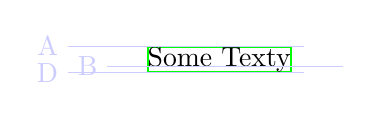
\begin{tikzpicture}
\node[inner sep=0,draw=green,thick] (text) {Some Texty};
\draw[-,blue!20] ($ (text.base west) - (0.5cm, 0) $) node[anchor=east] {B} -- ++(3cm, 0);
\draw[-,blue!20] ($ (text.base west) - (1.0cm, 0.2\baselineskip) $) node[anchor=east] {D} -- ++(3cm, 0);
\draw[-,blue!20] ($ (text.base west) - (1.0cm, -0.6\baselineskip) $) node[anchor=east] {A} -- ++(3cm, 0);
\end{tikzpicture}


Text nodes have 3 main lines used for aligning them. The base line \texttt{B} is just
the baseline of the text.

The line \texttt{A} is the ascender of the text.

The line \texttt{D} is the descender of the text.

Text nodes bounding box is always as heigh and wide as the text.


\subsection{Bracket}

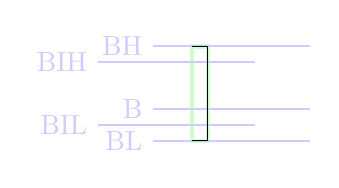
\begin{tikzpicture}

\draw (0, 0) coordinate (A)
  -- ++(0.2cm, 0) coordinate (B)
  -- ++(0, -0.2cm) coordinate (C)
  -- ++(0, -0.6cm) coordinate (D)
  -- ++(0, -0.2cm) coordinate (E)
  -- ++(0, -0.2cm) coordinate (F)
  -- ++(-0.2cm, 0) coordinate (G)
;

\begin{pgfonlayer}{background}
  \node[ultra thick,inner sep=0, fit={(A) (G) (B)},draw=green!20] {};
  \draw[thick,blue!20] ($ (A) - (0.5cm, 0) $) node[anchor=east] {BH} --+ (2cm, 0);
  \draw[thick,blue!20] ($ (G) - (0.5cm, 0) $) node[anchor=east] {BL} --+ (2cm, 0);
  \draw[thick,blue!20] ($ (D) - (0.7cm, 0) $) node[anchor=east] {B} --+ (2cm, 0);
  \draw[thick,blue!20] ($ (C) - (1.4cm, 0) $) node[anchor=east] {BIH} --+ (2cm, 0);
  \draw[thick,blue!20] ($ (E) - (1.4cm, 0) $) node[anchor=east] {BIL} --+ (2cm, 0);
\end{pgfonlayer}


\end{tikzpicture}


\texttt{BL} and \texttt{BH} denote the lowest and highest point of the bracket, respectively.

Brackets always have the same width. Brackets don't have a fixed height but get
their height based on their neighboring nodes in the same grid row. The
neighbors request a height and the height requested ist always the height
between \texttt{BIL} and \texttt{BIH}. There is a default margin between
\texttt{BIH} and \texttt{BH}, as well as between \texttt{BIL} and \texttt{BL}.

The baseline \texttt{B} is variable and depends on the neigbhours.

\subsection{Notes}

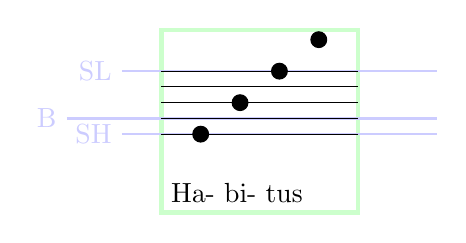
\begin{tikzpicture}
  \coordinate (ZLA0S) at (0,0);
  \coordinate (ZLA0E) at ($ (ZLA0S) + (\stafflinelength,0) $);
  \coordinate (ZLA1S) at ($ (ZLA0S) + (0,\stafflinemargin) $);
  \coordinate (ZLA1E) at ($ (ZLA1S) + (\stafflinelength,0) $);
  \coordinate (ZLA2S) at ($ (ZLA0S) + (0,2*\stafflinemargin) $);
  \coordinate (ZLA2E) at ($ (ZLA2S) + (\stafflinelength,0) $);
  \coordinate (ZLA3S) at ($ (ZLA0S) + (0,3*\stafflinemargin) $);
  \coordinate (ZLA3E) at ($ (ZLA3S) + (\stafflinelength,0) $);
  \coordinate (ZLA4S) at ($ (ZLA0S) + (0,4*\stafflinemargin) $);
  \coordinate (ZLA4E) at ($ (ZLA4S) + (\stafflinelength,0) $);

  \draw (ZLA0S) -- (ZLA0E);
  \draw (ZLA1S) -- (ZLA1E);
  \draw (ZLA2S) -- (ZLA2E);
  \draw (ZLA3S) -- (ZLA3E);
  \draw (ZLA4S) -- (ZLA4E);

  \draw[fill] ($ (ZLA0S) + (0.2*\stafflinelength, 0*\stafflinemargin) $) circle (0.1cm);
  \draw[fill] ($ (ZLA0S) + (0.4*\stafflinelength, 2*\stafflinemargin) $) circle (0.1cm);
  \draw[fill] ($ (ZLA0S) + (0.6*\stafflinelength, 4*\stafflinemargin) $) circle (0.1cm);
  \draw[fill] ($ (ZLA0S) + (0.8*\stafflinelength, 6*\stafflinemargin) $) circle (0.1cm) node (ND) {};

  \node[anchor=north west] (ZA-text) at ($ (ZLA0S) - (0, \textLineMargin) $) {Ha- bi- tus};

  \begin{pgfonlayer}{background}
    \node[ultra thick,inner sep=0, fit={(ZA-text.south west) (ZLA0E) (ND)},draw=green!20] {};
    \draw[thick,blue!20] ($ (ZLA1S) - (1.2cm, 0) $)   node[anchor=east] (B)  {B}  -- ++(4.7cm, 0);
    \draw[thick,blue!20] ($ (ZLA0S) - (0.5cm, 0) $)   node[anchor=east] (SH) {SH} -- ++(4cm, 0);
    \draw[thick,blue!20] ($ (ZLA4S) - (0.5cm, 0) $)   node[anchor=east] (SL) {SL} -- ++(4cm, 0);
  \end{pgfonlayer}

\end{tikzpicture}


The bounding box of the notes is the bounding box of all the text on the bottom as
well as the top notes.

There are three main lines used for alignment. The baseline \texttt{B} is always
the second staff line from the bottom. The other two import lines are \texttt{SL}
and \texttt{SH} which denote the lowest and highest staff line, respectively.

\section{Grid}

Grid nodes allow the layout of sub nodes. They can also themselves be the children of
other grid nodes. In this case, they are handled as a black box with no special
alignment lines.

\subsection{Horizontal}

The horizontal alignment of the grids is fairly simple. Their bouding box is used
and centered on the column by default. If the node has a justification (i.e. left,
center, right), the bounding box is shifted accordingly.

\subsection{Vertical}

The vertical alignment of nodes inside a row is harder. There are basically three cases
which depend on what the dominating node in the row is.

\subsubsection{Note dominated}

If there are one or more note-nodes in the row, one of them will be the
dominating node. It doesn't matter which one since all of them have the same
alignment lines after they are themselves aligned via their baselines.

All notes will be aligned according to the baseline of the dominating node. In
this case, other notes will be aligned by their second staff lines. Text nodes
will be aligned by their baseline. Opaque nodes like sub grids will be aligned
by the vertical center of their respective bounding boxes. Brackets
will be generated with the inner height (\texttt{BIL} to \texttt{BIH})
set to \texttt{SL} to \texttt{SH}. The baseline will be set to one fourth the
way between \texttt{BIL} and \texttt{BIH}.

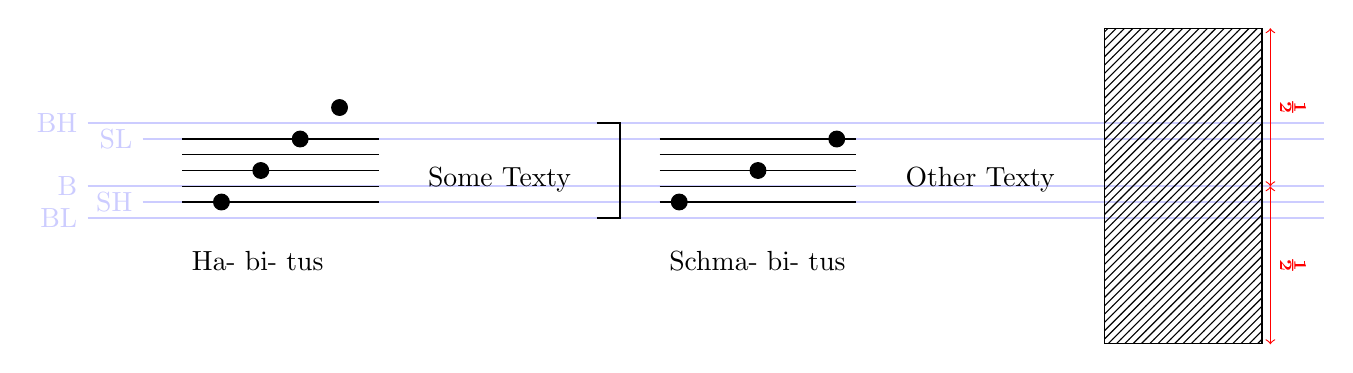
\begin{tikzpicture}
  \coordinate (ZLA0S) at (0,0);
  \coordinate (ZLA0E) at ($ (ZLA0S) + (\stafflinelength,0) $);
  \coordinate (ZLA1S) at ($ (ZLA0S) + (0,\stafflinemargin) $);
  \coordinate (ZLA1E) at ($ (ZLA1S) + (\stafflinelength,0) $);
  \coordinate (ZLA2S) at ($ (ZLA0S) + (0,2*\stafflinemargin) $);
  \coordinate (ZLA2E) at ($ (ZLA2S) + (\stafflinelength,0) $);
  \coordinate (ZLA3S) at ($ (ZLA0S) + (0,3*\stafflinemargin) $);
  \coordinate (ZLA3E) at ($ (ZLA3S) + (\stafflinelength,0) $);
  \coordinate (ZLA4S) at ($ (ZLA0S) + (0,4*\stafflinemargin) $);
  \coordinate (ZLA4E) at ($ (ZLA4S) + (\stafflinelength,0) $);

  \draw (ZLA0S) -- (ZLA0E);
  \draw (ZLA1S) -- (ZLA1E);
  \draw (ZLA2S) -- (ZLA2E);
  \draw (ZLA3S) -- (ZLA3E);
  \draw (ZLA4S) -- (ZLA4E);

  \draw[fill] ($ (ZLA0S) + (0.2*\stafflinelength, 0*\stafflinemargin) $) circle (0.1cm);
  \draw[fill] ($ (ZLA0S) + (0.4*\stafflinelength, 2*\stafflinemargin) $) circle (0.1cm);
  \draw[fill] ($ (ZLA0S) + (0.6*\stafflinelength, 4*\stafflinemargin) $) circle (0.1cm);
  \draw[fill] ($ (ZLA0S) + (0.8*\stafflinelength, 6*\stafflinemargin) $) circle (0.1cm);

  \node[anchor=north west] (ZA-text) at ($ (ZLA0S) - (0, \textLineMargin) $) {Ha- bi- tus};

  \node[anchor=base west] (first-text) at ($ (ZLA1E) + (0.5cm,0) $) {Some Texty};

  \coordinate (ZLB0S) at ($ (first-text.base east) + (1.0cm, -\stafflinemargin) $);
  \coordinate (ZLB0E) at ($ (ZLB0S) + (\stafflinelength,0) $);
  \coordinate (ZLB1S) at ($ (ZLB0S) + (0,\stafflinemargin) $);
  \coordinate (ZLB1E) at ($ (ZLB1S) + (\stafflinelength,0) $);
  \coordinate (ZLB2S) at ($ (ZLB0S) + (0,2*\stafflinemargin) $);
  \coordinate (ZLB2E) at ($ (ZLB2S) + (\stafflinelength,0) $);
  \coordinate (ZLB3S) at ($ (ZLB0S) + (0,3*\stafflinemargin) $);
  \coordinate (ZLB3E) at ($ (ZLB3S) + (\stafflinelength,0) $);
  \coordinate (ZLB4S) at ($ (ZLB0S) + (0,4*\stafflinemargin) $);
  \coordinate (ZLB4E) at ($ (ZLB4S) + (\stafflinelength,0) $);

  \draw (ZLB0S) -- (ZLB0E);
  \draw (ZLB1S) -- (ZLB1E);
  \draw (ZLB2S) -- (ZLB2E);
  \draw (ZLB3S) -- (ZLB3E);
  \draw (ZLB4S) -- (ZLB4E);

  \draw[fill] ($ (ZLB0S) + (0.1*\stafflinelength, 0*\stafflinemargin) $) circle (0.1cm);
  \draw[fill] ($ (ZLB0S) + (0.5*\stafflinelength, 2*\stafflinemargin) $) circle (0.1cm);
  \draw[fill] ($ (ZLB0S) + (0.9*\stafflinelength, 4*\stafflinemargin) $) circle (0.1cm);

  \node[anchor=north west] (ZB-text) at ($ (ZLB0S) - (0, \textLineMargin) $) {Schma- bi- tus};

  \draw[-,thick] ($ (ZLB4S) - (0.8cm, -\stafflinemargin) $) coordinate (BracketA)
    -- ++ (0.3cm,0) coordinate (BracketB)
    -- ++ (0,0.-6*\stafflinemargin) coordinate (BracketC)
    -- ++(-0.3cm, 0) coordinate (BracketD)
  ;

  \node[anchor=base west] (second-text) at ($ (ZLB1E) + (0.5cm,0) $) {Other Texty};

  \node[
      draw,
      minimum width=2cm,
      minimum height=4cm,
      anchor=west,
      pattern=north east lines
    ] (sub grid) at ($ (second-text.base east) + (0.5cm, 0) $) {};

  \draw[red,<->] ($ (sub grid.north east) +(0.1cm, 0) $)
    -- ($ (sub grid.north east)!0.5!(sub grid.south east) + (0.1cm, 0) $) node[above, midway,rotate=-90] {½}
  ;
  \draw[red,<->] ($ (sub grid.north east)!0.5!(sub grid.south east) + (0.1cm, 0) $)
    -- ($ (sub grid.south east) +(0.1cm, 0) $) node[above, midway,rotate=-90] {½}
  ;
   


  \begin{scope}[on background layer]
    \draw[thick,blue!20] ($ (ZLA1S) - (1.2cm, 0) $)   node[anchor=east] (B)  {B}  -- ++(15.7cm, 0);
    \draw[thick,blue!20] ($ (ZLA0S) - (0.5cm, 0) $)   node[anchor=east] (SH) {SH} -- ++(15cm, 0);
    \draw[thick,blue!20] ($ (ZLA4S) - (0.5cm, 0) $)   node[anchor=east] (SL) {SL} -- ++(15cm, 0);
    \draw[thick,blue!20] (B.east |- BracketA) node[anchor=east] (BH) {BH} -- ++(15.7cm, 0);
    \draw[thick,blue!20] (B.east |- BracketD) node[anchor=east] (BL) {BL} -- ++(15.7cm, 0);
  \end{scope}

\end{tikzpicture}


\subsubsection{Text dominated}

In case there are no note-nodes in the row, text nodes will be the dominating.
Which one, again, doesn't matter, since they are aligned via baseline and
then have the same ascender/descener lines after that.

The layouting will work as above, only brackets are generated differently. The inner
height of the bracket (\texttt{BIL} to \texttt{BIH}) will be set to the height
of the text nodes in the row, i.e. to \texttt{D} to \texttt{A}. The baseline will
be \( \frac{B - A}{D - A} \) the way between \texttt{BIL} and \texttt{BIH}.

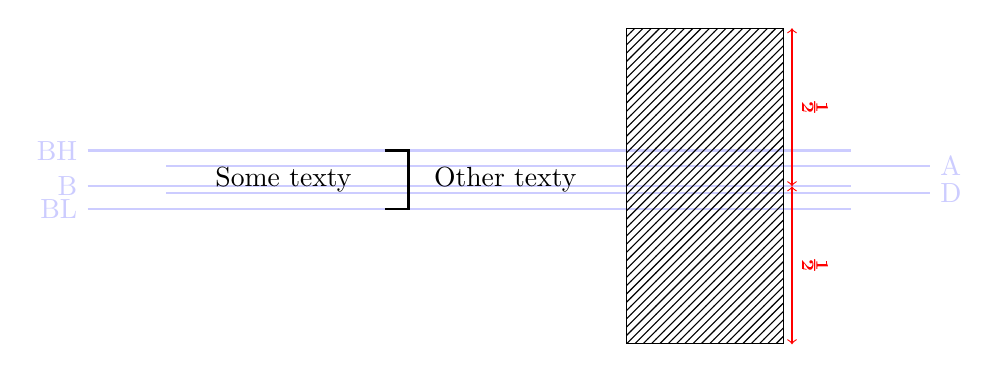
\begin{tikzpicture}

\node[anchor=base] (TA) {Some texty};
\coordinate (TAA) at ($ (TA.base west) - (0, -0.6 *\baselineskip) $);
\coordinate (TAD) at ($ (TA.base west) - (0, 0.2 *\baselineskip) $);

\node[anchor=base west] at ($ (TA.base east) + (0.8cm, 0) $) (TB) {Other texty};
\coordinate (TBA) at ($ (TB.base west) - (0, -0.6 *\baselineskip) $);
\coordinate (TBD) at ($ (TB.base west) - (0, 0.2 *\baselineskip) $);

\draw[-,thick] ($ (TBA) - (0.5cm, -\stafflinemargin) $) coordinate (BracketA)
  -- ++ (0.3cm,0) coordinate (BracketB)
  -- ($ (TBD) - (0.2cm, \stafflinemargin) $) coordinate (BracketC)
  -- ++(-0.3cm, 0) coordinate (BracketD)
;

\node[
    draw,
    minimum width=2cm,
    minimum height=4cm,
    anchor=west,
    pattern=north east lines
  ] (sub grid) at ($ (TB.base east) + (0.5cm, 0) $) {};

  \draw[red,<->] ($ (sub grid.north east) +(0.1cm, 0) $)
    -- ($ (sub grid.north east)!0.5!(sub grid.south east) + (0.1cm, 0) $) node[above, midway,rotate=-90] {½}
  ;
  \draw[red,<->] ($ (sub grid.north east)!0.5!(sub grid.south east) + (0.1cm, 0) $)
    -- ($ (sub grid.south east) +(0.1cm, 0) $) node[above, midway,rotate=-90] {½}
  ;

\begin{scope}[on background layer]
  \draw[thick,blue!20] ($ (TA.base west) - (1.5cm, 0) $) node[anchor=east] (B)  {B}  -- ++(9.7cm, 0);
  \draw[thick,blue!20] ($ (TA.base west) - (0.5cm, -0.6 *\baselineskip) $) -- ++(9.7cm, 0) node[anchor=west] {A};
  \draw[thick,blue!20] ($ (TA.base west) - (0.5cm, 0.2 *\baselineskip) $) -- ++(9.7cm, 0)  node[anchor=west] {D};
  \draw[thick,blue!20] (B.east |- BracketA) node[anchor=east] (BH) {BH} -- ++(9.7cm, 0);
  \draw[thick,blue!20] (B.east |- BracketD) node[anchor=east] (BL) {BL} -- ++(9.7cm, 0);
\end{scope}

\end{tikzpicture}


\subsubsection{Undominated}

If only opqaue nodes are left in the row, they will all be aligned by
their vertical center. Brackets will always have some default height, left
as an implementation detail.

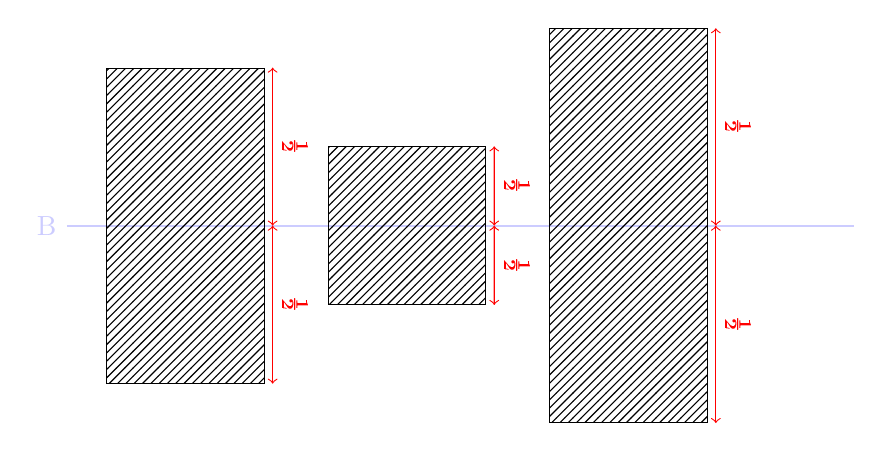
\begin{tikzpicture}

\node[
    draw,
    minimum width=2cm,
    minimum height=4cm,
    anchor=west,
    pattern=north east lines
  ] (SG1) at (0, 0) {};

  \draw[red,<->] ($ (SG1.north east) +(0.1cm, 0) $)
    -- ($ (SG1.north east)!0.5!(SG1.south east) + (0.1cm, 0) $) node[above, midway,rotate=-90] {½}
  ;
  \draw[red,<->] ($ (SG1.north east)!0.5!(SG1.south east) + (0.1cm, 0) $)
    -- ($ (SG1.south east) +(0.1cm, 0) $) node[above, midway,rotate=-90] {½}
  ;


\node[
    draw,
    minimum width=2cm,
    minimum height=2cm,
    anchor=west,
    pattern=north east lines
  ] (SG2) at ($ (SG1.east) + (0.8cm, 0) $) {};

  \draw[red,<->] ($ (SG2.north east) +(0.1cm, 0) $)
    -- ($ (SG2.north east)!0.5!(SG2.south east) + (0.1cm, 0) $) node[above, midway,rotate=-90] {½}
  ;
  \draw[red,<->] ($ (SG2.north east)!0.5!(SG2.south east) + (0.1cm, 0) $)
    -- ($ (SG2.south east) +(0.1cm, 0) $) node[above, midway,rotate=-90] {½}
  ;


\node[
    draw,
    minimum width=2cm,
    minimum height=5cm,
    anchor=west,
    pattern=north east lines
  ] (SG3) at ($ (SG2.east) + (0.8cm, 0) $) {};

  \draw[red,<->] ($ (SG3.north east) +(0.1cm, 0) $)
    -- ($ (SG3.north east)!0.5!(SG3.south east) + (0.1cm, 0) $) node[above, midway,rotate=-90] {½}
  ;
  \draw[red,<->] ($ (SG3.north east)!0.5!(SG3.south east) + (0.1cm, 0) $)
    -- ($ (SG3.south east) +(0.1cm, 0) $) node[above, midway,rotate=-90] {½}
  ;

\begin{scope}[on background layer]
  \draw[thick,blue!20] ($ (SG1.west) - (0.5cm, 0) $) node[anchor=east] (B)  {B}  -- ++(10.0cm, 0);
\end{scope}

\end{tikzpicture}


\end{document}
